\chapter*{Chapter 2}
\markboth{Chapter 2 }{ EIT systems in biomedical applications and proposed contribution} %pour afficher l'entete
\addcontentsline{toc}{chapter}{II EIT systems in biomedical applications and proposed contribution}

\textbf {\Huge EIT systems in biomedical applications and proposed contribution} \\ 

\setcounter{chapter}{2}
\setcounter{section}{0}

%\end{chapter1}
\section{Introduction}
Electrical Impedance Tomography (EIT) is a non-invasive imaging technique that reconstructs the conductivity distribution in a body from small electrical currents introduced into the body and measured surface voltages. Due to the safety, portability, and low cost of EIT, it has gained increasing attention for biomedical applications, such as monitoring the lung, brain imaging, and cancer detection. This chapter overviews the fundamentals of EIT, reports recent advances in multi-frequency EIT systems, and discusses current limitations
and introduces our proposed method for better multi-frequency EIT performance.


\section{Fundamentals of EIT}
Electrical Impedance Tomography (EIT) is a tomographic method that reconstructs the
image of the internal electrical properties of a medium, typically biological tissue, from surface
electrical measurements. It relies on injecting small alternating currents into the body through
body surface electrodes and measuring the resultant voltages. The spatial distribution of
electrical conductivity and permittivity inside the body affects
these measurements, which can enable image reconstruction\cite{WikipediaEIT}
\subsection{Measurement protocols}
\begin{itemize}
\item
For Electrical Impedance Tomography (EIT), a ring of electrodes is
arranged evenly around the region to be investigated, e.g., the chest
or forearm. In our system, we used 16 circularly disposed electrodes.
To obtain data, a small, known alternating current (AC) is injected
between two selected electrodes—typically adjacent or opposite pairs. This injected current propagates through
the tissues, and the resulting voltage differences are sensed by the remainder of
electrodes. By successively varying the pair of electrodes used to inject the current and measure
the resulting voltages at other electrodes, we are able to get a full set of measurements
that sample the internal distribution of electrical impedance. These are acquired as
input for image reconstruction algorithms in order to produce conductivity maps of
the target tissue.
This technique allows us to study the electrical properties of the tissue, as different types of tissues affect current conduction in typical ways because of their individual conductivity and permittivity.




\item
The array of electrodes used for injecting current and for sensing voltage is called the measurement pattern. Different patterns control the sensitivity distribution, resolution, and the depth of the reconstructed image\cite{MDPI2021}:
\begin{itemize}
\item Adjacent pattern: Current is injected through a pair of neighboring electrodes, and voltage measurements are collected from the remaining electrode
pairs. This approach is widely used due to its simplicity and ability to provide good
spatial sensitivity near the boundary.
\item Opposite pattern: Current is passed between opposite electrodes
(e.g., E1–E9 in a 16-electrode system), improving sensitivity in the central region.
\item Skip patterns: Current is passed between electrodes skipped by one or more intermediate electrodes. As an example, skip-1 uses E1–E3, skip-2 uses E1–E4, etc. These patterns offer a trade-off between central and boundary sensitivity.\cite{Adler2016}\\
In this project, we selected the adjacent injection to maximize boundary sensitivity .
\end{itemize}

In this work, the adjacent injection protocol was chosen to maximize boundary sensitivity, as illustrated in Figure~\ref{fig:enter-label}.
\begin{figure}[H]
    \centering
    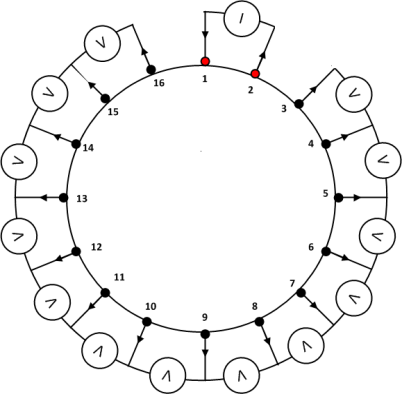
\includegraphics[width=0.4\linewidth]{imagess/AAA.png}
    \caption{EIT adjacent injection protocol using 16 electrodes.\cite{Angelucci2021}}
    \label{fig:enter-label}
\end{figure}
\end{itemize}
\subsection{Mathematical formulation}
After defining the measurement protocols, we now explore the mathematical challenges inherent in reconstructing conductivity images from voltage measurements.\\
Once voltage and current measurements have been collected from different current injection patterns, the next task in EIT is the reconstruction of the internal conductivity structure of the target region. The process is called solving the inverse problem.
In EIT, the forward problem is well-defined: with a known conductivity dist-
tribution, one can calculate the voltages on electrodes using Maxwell's equations

The inverse problem is the reverse: solving for conductivity distribution from known voltages.
The inverse problem in EIT is inherently:
\begin{itemize}
    \item \textbf{Nonlinear} : Conductivity and measured voltages are nonlinearly related.
    \item \textbf{Ill-posed} : Small measurement noise can create large errors in the reconstructed
image; multiple distributions of conductivity may fit the same voltage data.
    \item \textbf{Underdetermined} :  the unknowns (internal values of conductivity) are typically much larger than the number of measurements available.
\end{itemize}

The relationship can be expressed as \cite{Seo2019}:
\begin{equation}
V = F(\sigma) + \varepsilon
\label{eq:forward_model}
\end{equation}
where:
\begin{itemize}
    \item $V$ = vector of measured voltages
    \item $\sigma$ = conductivity distribution to be estimated
    \item $F$ = nonlinear forward model
    \item $\varepsilon$ = measurement noise
\end{itemize}
Figure~\ref{fig:enter-label} illustrates a schematic representation of the Electrical Impedance Tomography (EIT) process, showing how current is injected, boundary voltages are measured and then the image is reconstructed.


\begin{figure}[H]
    \centering
    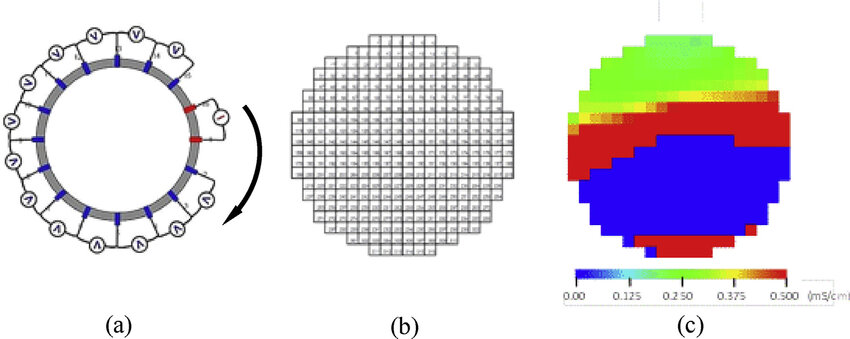
\includegraphics[width=0.8\linewidth]{imagess/Schematics-showing-a-the-adjacent-current-injection-pattern-for-a-circular-16-electrode.png}
    \caption{Schematic representation of the EIT process.\cite{Hou2016}}
    \label{fig:enter-label}
\end{figure}


\section{Frequency-dependent impedance properties of biological tissues}
Biological tissues are frequency dependent in their impedance properties, due in large part to cell membranes, intracellular and extracellular fluids, and tissue composition. At low frequencies, current travels mostly through the extracellular space because cell membranes act as capacitors, blocking direct current access into the cells. As frequency is increased, the membrane capacitive reactance decreases, and current can enter the intracellular space.

This property is exploited in \textit{multi-frequency EIT} (MFEIT) to provide improved tissue characterization and discrimination. By having EIT data at multiple frequencies, it is possible to discriminate between tissues or to identify physiological changes that would not be visible with single-frequency data.

This frequency-dependent response is particularly useful for biomedical applications when detecting pathological changes such as edema, ischemia, or tumor development since such conditions often alter the dielectric properties of tissues at certain frequency \cite{Bera2017}.
\\The figure 2.7 illustrates how the electrical impedance of biological tissues changes with frequency, showcasing the characteristic frequency-dependent behavior exploited in multi-frequency EIT.
\begin{figure}[H]
    \centering
    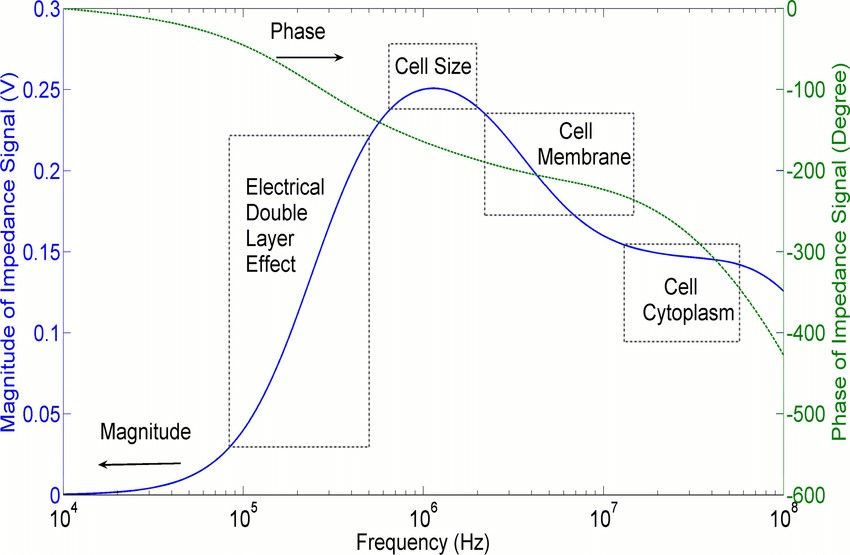
\includegraphics[width=0.8\linewidth]{imagess/8dhl6ptn.png}
    \caption{Measured tissue impedance as a function of frequency\cite{Sun2008}}
    \label{fig:enter-label}
\end{figure}

\end{itemize}
\section{Multi-frequency EIT methods}
In order to evaluate the progress and challenges of multi-frequency EIT, it is essential to review and compare the main systems proposed in the literature. Several implementations have been reported with differences in electrode configurations, excitation strategies, frequency ranges, and data acquisition methods. A comparative analysis highlights the advantages and trade-offs of these approaches, providing a reference against which the proposed system can be positioned.
\subsection{Benchmarking}
Multi-frequency Electrical Impedance Tomography (MFEIT) extends the capabilities of conventional single-frequency EIT by acquiring data over a range of frequencies. 
This approach leverages the frequency-dependent electrical properties of biological tissues, enabling improved differentiation between tissue types, enhanced image reconstruction, and the extraction of additional physiological information. 

\begin{table}[H]
\centering
\caption{ Multi-frequency EIT systems }
\resizebox{\textwidth}{!}{%
\begin{tabular}{|m{1cm}|m{2cm}|m{3.5cm}|m{3.5cm}|m{2.5cm}|m{2.5cm}|m{2.5cm}|m{3cm}|m{3.5cm}|}
\hline
\textbf{Ref} & \textbf{Electrodes} & \textbf{Frequency range \& number} & \textbf{Data type} & \textbf{ADC resolution} & \textbf{MCU} & \textbf{Excitation type} & \textbf{Acquisition time} & \textbf{Application} \\ \hline
\cite{Klosowski2025} & 32 & 100 kHz, 50 kHz, 10 kHz, 3 freqs & Resistive, Reactive & – & Dual-core ARM Cortex-A9 & Single sine wave & – & Industrial \\ \hline
\cite{LiWang2025} & – & 10–100 kHz & Magnitude, Phase & – & – & Sequential MF & 10–100 fps & Medical, Industrial, Geo \\ \hline
\cite{Chen2021} & 16 & 10–100 kHz, 5 freqs & Voltage & – & – & sequential MF & – & Biomedical \\ \hline
\cite{Yang2022} & 16 & 100 kHz–1 MHz & Amplitude, Phase & 12-bit & DSP TMS320 F28335 & Sequential MF & 208 voltages/cycle & Biomedical, Industrial, Agricultural \\ \hline
\cite{Zhu2024} & 12 & 10 kHz–1 MHz, 3 freqs & Impedance & 16-bit & STM32F103 & Sequential MF & 15 fps & Biomedical \\ \hline
\cite{Sensors2019} & 16 & 60–960 kHz, 2 freqs & I/Q Demodulation & 14-bit & Virtex-6 FPGA & Simultaneous MF & 32.8–131 fps & Lung, Cardiac, Perfusion monitoring \\ \hline
\end{tabular}%
}

\label{tab:eit-comparison}
\end{table}


Table 2.1 summarizes recent multi-frequency EIT implementations across various applications, highlighting differences in electrode configurations, frequency ranges, excitation types, ADC resolutions, and acquisition methods. While these systems demonstrate progress toward multi-frequency impedance imaging, the analysis reveals persistent trade-offs between acquisition speed, frequency coverage, measurement precision, and application-specific requirements. Notably, the majority of biomedical-focused systems rely on sequential frequency excitation, limiting temporal resolution and robustness in dynamic environments. Additionally, ADC resolution and simultaneous acquisition capabilities vary widely, indicating significant room for improvement to meet the stringent demands of real-time clinical monitoring.

\subsection{Limitations }
In Electrical Impedance Tomography (EIT), conventional systems often operate at a single frequency (monofrequency). While simple and fast, monofrequency measurements cannot capture frequency-dependent tissue properties, such as the difference between extracellular and intracellular conductivity. This limits the ability to distinguish different tissue types or monitor complex physiological processes.

To address this, many systems use sequential multi-frequency excitation, where currents are applied one frequency at a time and the resulting voltages are measured before moving to the next frequency ([12], [13], [15], [21]; see Table 2.1). Sequential systems are relatively easy to implement, but they have several limitations. First, the overall acquisition time increases proportionally with the number of frequencies, which can be a problem in fast-changing biological conditions. Second, motion artifacts may occur between frequencies: physiological movements, such as heartbeats, breathing, or patient motion, can alter the measured voltages from one frequency to the next. These temporal inconsistencies create errors and distortions in the reconstructed impedance images, reducing spatial accuracy and reliability.

Some advanced systems, such as [26], implement simultaneous acquisition but are limited to only two discrete frequencies. While better than sequential methods, this still restricts the frequency range and reduces the ability to exploit the full spectral information of biological tissues.

The main challenge in multi-frequency EIT is therefore to develop systems that can excite and measure multiple frequencies at the same time. Simultaneous multi-frequency EIT reduces overall measurement time, eliminates motion artifacts between frequencies, and improves imaging accuracy and reliability. This is essential for dynamic, real-time biomedical applications, such as monitoring muscle activity, lung function, or other rapid physiological processes.

\section{Proposed approach for enhancement of multi- frequency EIT}

To overcome the limitations of existing multi-frequency EIT systems, this work proposes a simultaneous multi-frequency excitation and measurement strategy designed to improve temporal resolution and enhance diagnostic precision. Unlike traditional sequential frequency sweeps, the simultaneous approach enables real-time acquisition of frequency-dependent tissue information, thereby minimizing motion artifacts and better capturing rapid physiological changes.  

The proposed system architecture is organized around several key building blocks. A dedicated current source (VCCS) generates stable multi-frequency excitation signals that are applied to a set of boundary electrodes through multiplexers and demultiplexers. The selection of electrode pairs for current injection and voltage measurement is controlled dynamically, enabling flexible measurement patterns. The STM32G474 microcontroller forms the core of the system, integrating a high-speed DAC for excitation signal generation and high-resolution ADCs for voltage acquisition. Signal conditioning modules are employed to ensure measurement integrity by filtering noise, stabilizing signals, and matching impedance before digitization. The acquired signals are then processed in real time to separate frequency components, compute impedance values, and prepare the data for higher-level analysis. This integrated architecture makes the system compact, efficient, and suitable for portable biomedical applications.  


A central innovation in the proposed approach lies in the excitation strategy. Instead of using simple sinusoidal signals, a specially optimized multisine stimulus is employed. The frequency components of this multisine are carefully selected using an optimization algorithm that balances two criteria: (i) maximizing spectral coverage across the frequencies of interest, and (ii) minimizing interference and harmonic distortion between components. The optimization process ensures that injected signals remain orthogonal and well-separated, enabling accurate frequency-domain analysis even under simultaneous operation. Compared to sequential frequency sweeps, this optimized multisine excitation significantly reduces measurement time while increasing robustness against motion artifacts, thus paving the way for precise and real-time biomedical imaging.  

The subsequent chapters present the detailed system design and implementation. Chapter~3 elaborates on the architecture, hardware realization, and signal conditioning techniques, while Chapter~4 discusses the signal processing methods and validates the proposed approach through experimental results.

\section{Conclusion}

In this chapter, a comprehensive description of existing multi-frequency Electrical Impedance Tomography systems was presented, indicating their current shortcomings in terms of temporal resolution, measurement accuracy, and susceptibility to motion artifacts. To address these problems, a novel idea of simultaneous multi-frequency excitation and high-resolution data acquisition using the 16-bit ADC of STM32G4 microcontroller was proposed. The use of an optimized multisine excitation signal further develops the potential of the system since it enables simultaneous frequency measurements in an efficient and accurate way.
This proposed approach offers a sound foundation for higher fidelity images and
biomedical real-time processing. The design and implementation details will be covered
in the following chapter.

